\documentclass[]{article}

\usepackage{graphicx} %for å inkludere grafikk
\usepackage{verbatim} %for å inkludere filer med tegn LaTeX ikke liker
\usepackage{tabularx}
\usepackage{booktabs}
\usepackage{amsmath}
\usepackage{float}
\usepackage{color}
\usepackage{listings}
\usepackage{physics}
\usepackage{hyperref}
\usepackage{subfig}
\usepackage{mhchem}
\usepackage{natbib}
%opening
\title{}
\author{}

\begin{document}
	
\title{FREYA Report after Berkeley visit}
\author{Dorthea Gjestvang}
\date{January 2018}

\maketitle

\section{Introduction}

\section{Theory: FREYA}

\section{Method}

\section{Results}

\subsection{Spontaneous fission of Cf252 }

The four first neutron factorial moments is shown in table \ref{tab:Cf252_n_moments}, and the dependence of the mean neutron multiplicity $\nu$ and the photon multiplicity $N_{\gamma}$ on the parameters dTKE and x  can be seen in Table \ref{tab:dependence_on_dTKE} and \ref{tab:dependence_on_x} respectively. The dependence of $N_{\gamma}$ on $c_s$ is shown in Table \ref{tab:dependence_on_c}.

The fragment and product mass distribution is shown in Figure \ref{fig:Cf252_sf_fragment_product_yield}, and the mean kinetic energy of the fragments as a function of mass is shown in Figure \ref{fig:Cf252_sf_mean_fragment_kinetic_enery_function_of_fragment_mass_number}. The multiplicity distribution and spectral shape of the emmited neutrons and photons respectively is shown in Figure \ref{fig:Cf252_sf_total_n_mult}, \ref{fig:Cf252_sf_neutron_spectral_shape}, \ref{fig:Cf252_sf_total_ph_mult} and \ref{fig:Cf252_sf_photons_spectral_shape}. The angular correlation between pairs of emmited neutrons are shown in Figure \ref{fig:Cf252_sf_n_n_ang_corr}.


\begin{table} [H]
	\centering
	\caption{The four first neutron factorial moments from the spontaneous fission of Cf252}
	\begin{tabularx}{\textwidth}{XX} \hline
		\label{tab:Cf252_n_moments}
		Moment & Value \\ \hline
		1 & 3.74896 \\
		2 & 12.0088\\
		3 & 32.1299\\
		4 & 69.7771\\ 
	\end{tabularx}
\end{table}

\begin{table} [H]
	\centering
	\caption{The dependence of $\overline{\nu}$  and $\overline{\nu_1}$, $\overline{\nu_2}$ and $\overline{N}_{\gamma}$ on dTKE, when x=1.27 is held constant}
	\begin{tabularx}{\textwidth}{XXXXXX} \hline
		\label{tab:dependence_on_dTKE}
		Variable & dTKE = 0.01&dTKE = 0.32 &dTKE=0.52 (default) & dTKE= 1.00 & dTKE= 1.52\\ \hline
		$\overline{\nu}$ & 3.80868 & 3.77398 & 3.74896 & 3.68827 & 3.62737\\
		$\overline{\nu_1}$ & 2.20929 & 2.18963  & 2.17103& 2.14226 & 2.10651 \\
		$\overline{\nu_2}$ & 1.59939 &1.58435 & 1.57793 & 1.54601 &  1.52086\\ 
		$\overline{N}_{\gamma}$ & 7.70655 & 7.67067 & 7.68255 & 7.66869 & 7.65534\\
		\hline
	\end{tabularx}
\end{table}

\begin{table} [H]
	\centering
	\caption{The dependence of $\overline{\nu}$, $\overline{\nu_1}$, $\overline{\nu_2}$ and $\overline{N}_{\gamma}$ on x, when dTKE=0.52 is held constant}
	\begin{tabularx}{\textwidth}{XXXXXX} \hline
		\label{tab:dependence_on_x}
		Variable & x = 0.80 & x  = 1.00 & x = 1.27 (default) & x = 1.30 & x= 1.40\\ \hline
		$\overline{\nu}$ & 3.74887 & 3.77249 & 3.74896 & 3.74645 & 3.71148\\
		$\overline{\nu_1}$ & 1.34564 & 1.70729  & 2.17103 & 2.22821 & 2.38825 \\
		$\overline{\nu_2}$ & 2.40323  & 2.0652 & 1.57793 & 1.51824 & 1.32323 \\ 
		$\overline{N}_{\gamma}$ & 7.63944 & 7.65454 & 7.68255 & 7.69108 & 7.70245\\
		\hline
	\end{tabularx}
\end{table}

\begin{table} [H]
	\centering
	\caption{The dependence of  $\overline{N}_{\gamma}$ on cs}
	\begin{tabularx}{\textwidth}{XXXXXX} \hline
		\label{tab:dependence_on_c}
		 & cs=0.77 & cs= 0.82 & cs=0.87 (default) & cs= 0.97 & cs= 1.07 \\ \hline
		$\overline{N}_{\gamma}$ & 7.4015 & 7.53367 & 7.68255 & 7.95058 & 8.23856 \\
		\hline
	\end{tabularx}
\end{table}

\begin{figure} [H]
	\centering
	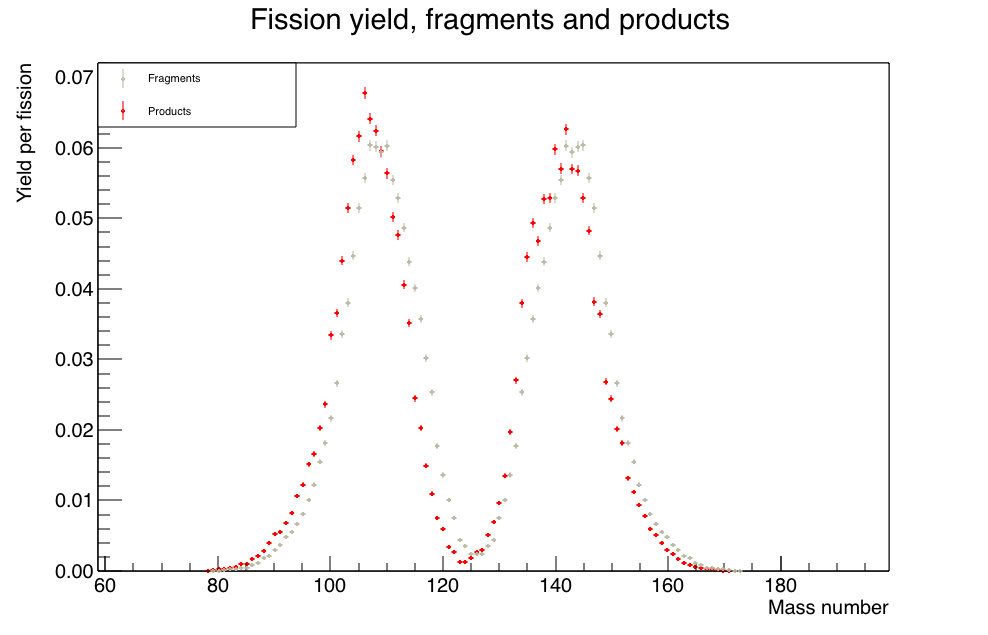
\includegraphics[scale=0.37]{Cf252_sf_fragment_product_yield.png}
	\caption{The fragment and product yield from the spontaneous fission of Cf252}
	\label{fig:Cf252_sf_fragment_product_yield}
\end{figure}

\begin{figure} [H]
	\centering
	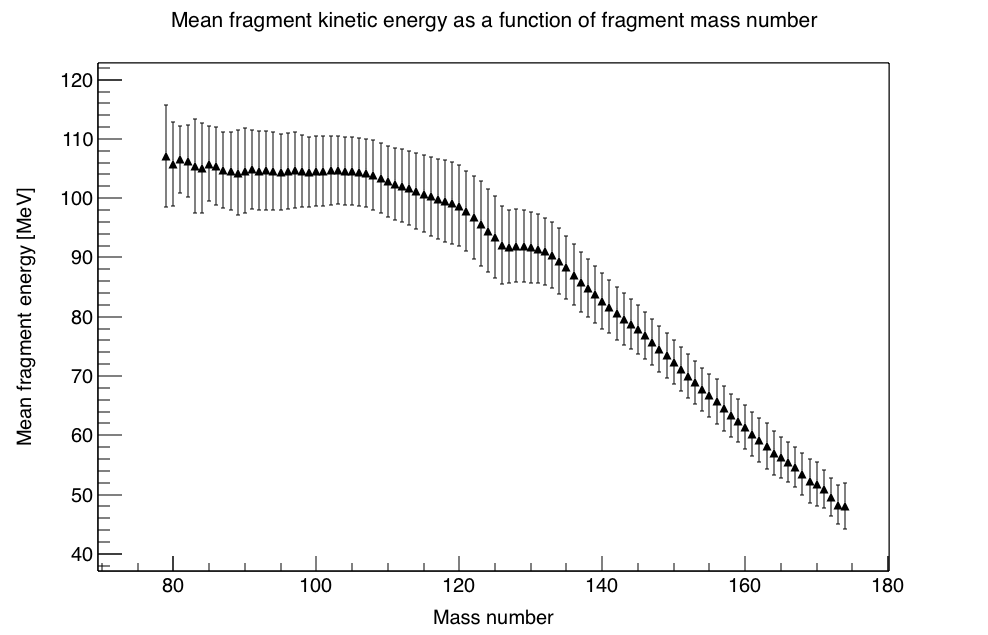
\includegraphics[scale=0.37]{Cf252_sf_mean_fragment_kinetic_enery_function_of_fragment_mass_number.png}
	\caption{The mean fragment energy as a function of fragment mass, from the spontaneous fission of Cf252}
	\label{fig:Cf252_sf_mean_fragment_kinetic_enery_function_of_fragment_mass_number}
\end{figure}

\begin{figure} [H]
	\centering
	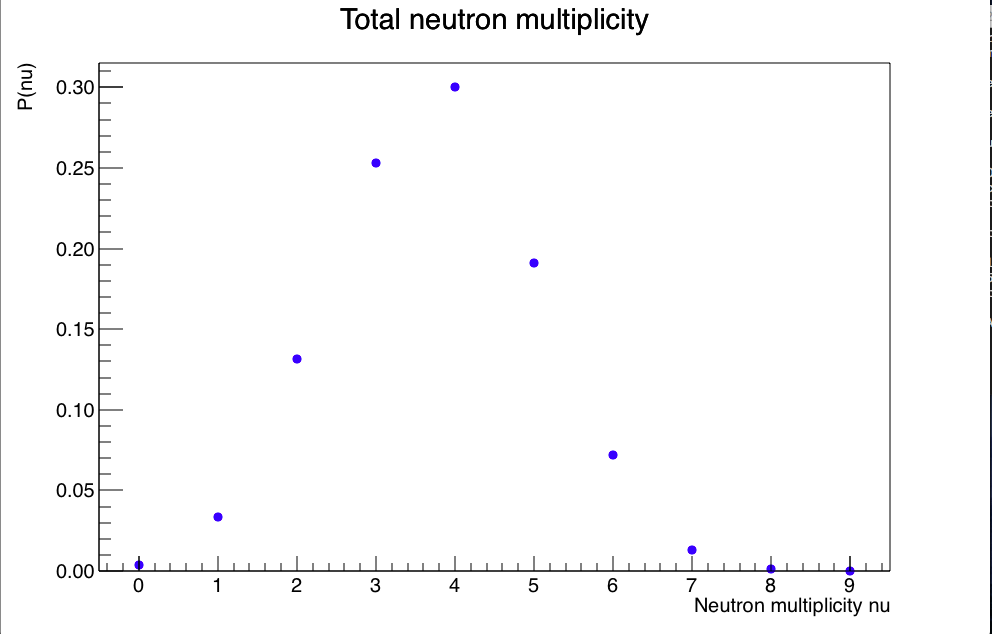
\includegraphics[scale=0.36]{Cf252_sf_total_n_mult.png}
	\caption{The multiplicity distribution of neutrons from the spontaneous fission of Cf252}
	\label{fig:Cf252_sf_total_n_mult}
\end{figure}

\begin{figure} [H]
	\centering
	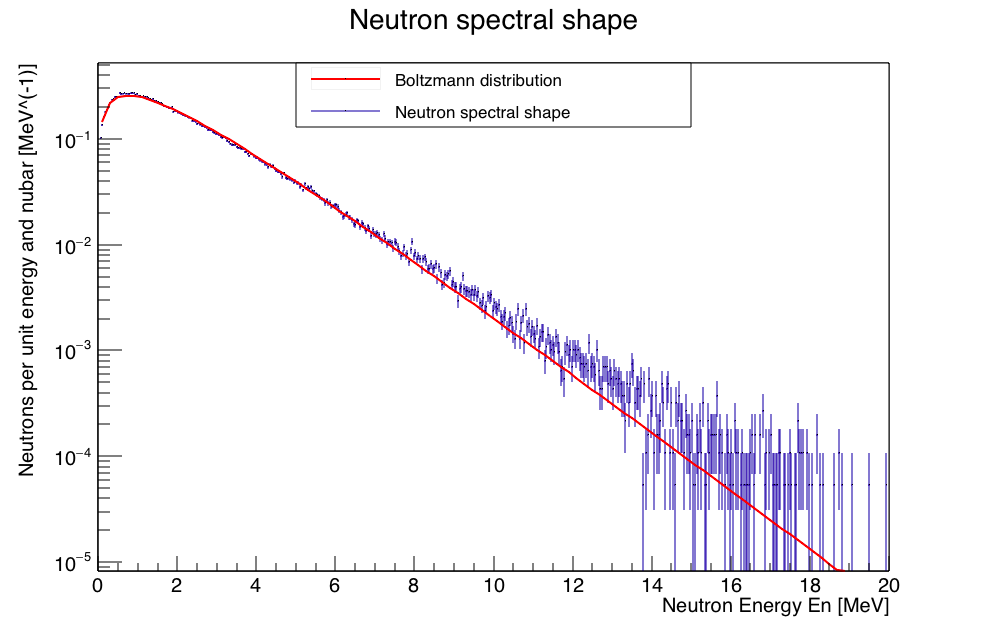
\includegraphics[scale=0.36]{Cf252_sf_neutron_spectral_shape.png}
	\caption{The spectral shape of neutrons from the spontaneous fission of Cf252, compared to a fitted Boltzmann distribution}
	\label{fig:Cf252_sf_neutron_spectral_shape}
\end{figure}

\begin{figure} [H]
	\centering
	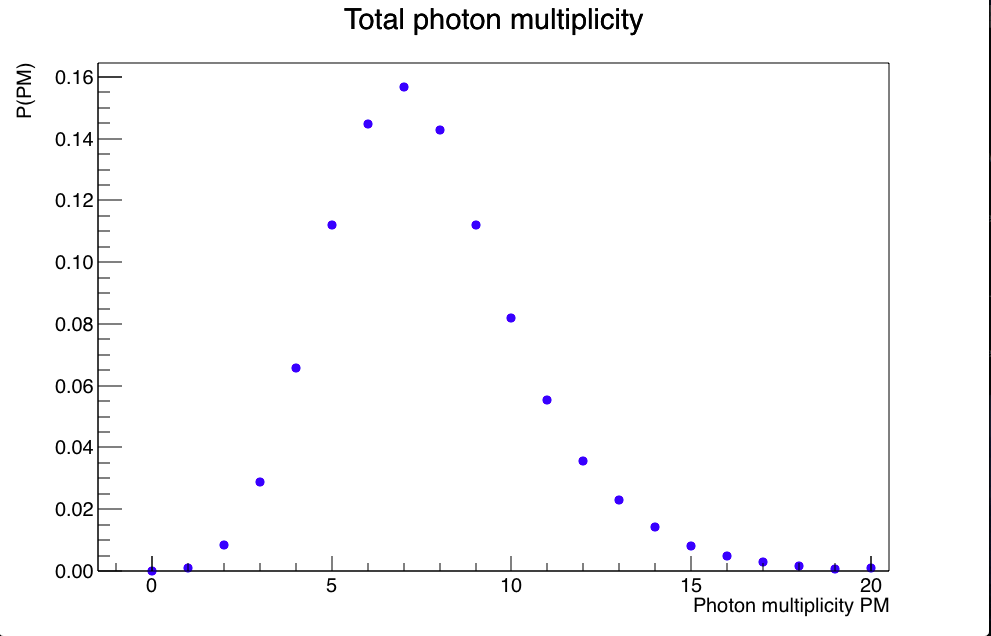
\includegraphics[scale=0.36]{Cf252_sf_total_ph_mult.png}
	\caption{The multiplicity distribution of photons from the spontaneous fission of Cf252}
	\label{fig:Cf252_sf_total_ph_mult}
\end{figure}

\begin{figure} [H]
	\centering
	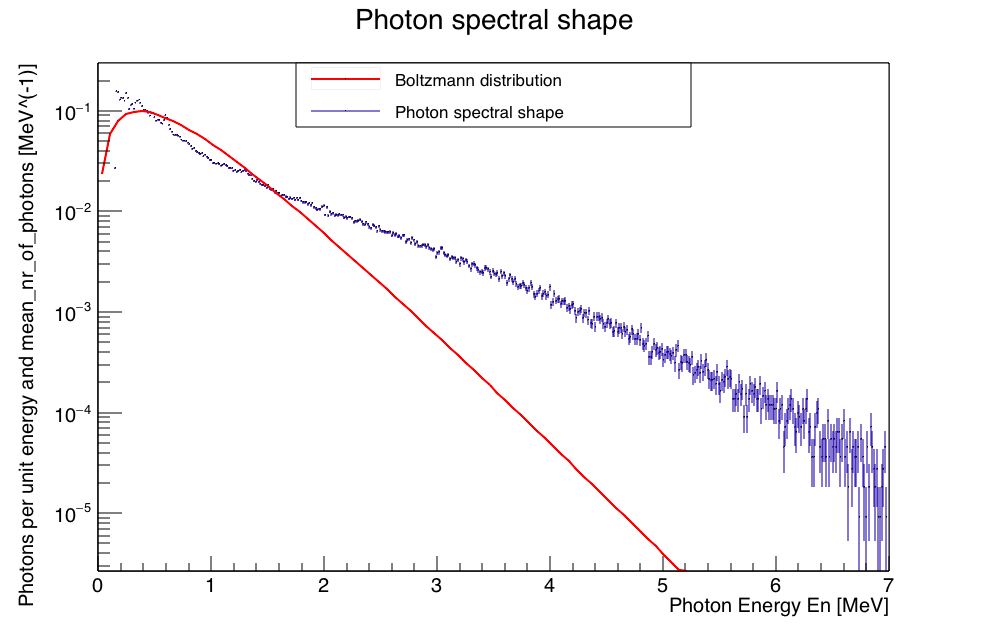
\includegraphics[scale=0.36]{Cf252_sf_photons_spectral_shape.png}
	\caption{The spectral shape of photons from the spontaneous fission of Cf252, compared to a fitted Boltzmann distribution}
	\label{fig:Cf252_sf_photons_spectral_shape}
\end{figure}
	
\begin{figure} [H]
	\centering
	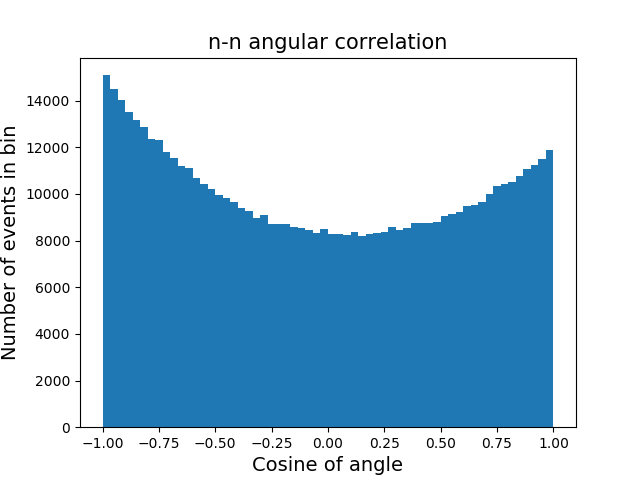
\includegraphics[scale=0.7]{Cf252_sf_n_n_ang_corr.png}
	\caption{The angulare correlation between pairs of emmited neutrons from the spontaneous fission of Cf252}
	\label{fig:Cf252_sf_n_n_ang_corr}
\end{figure}
	
\subsection{Thermal neutron induced fission of U235}

The four first neutron factorial moments is shown in table \ref{tab:U235_n_moments}. The fragment and product distribution is shown in Figure \ref{fig:U235_fragment_product_distribution}. 

The multiplicity distribution and spectral shape of the emmited neutrons and photons respectively is shown in Figure \ref{fig:U235_n_mult}, \ref{fig:U235_n_spectral_shape}, \ref{fig:U235_ph_mult} and \ref{fig:U235_ph_spectral_shape}. The angular correlation between pairs of emmited neutrons are shown in Figure \ref{fig:U235_n_n_ang_corr}.

\begin{table} [H]
	\centering
	\caption{Neutrons, first four factorial moments, from thermal neutron-induced fission of U235 }
	\begin{tabularx}{\textwidth}{XX} \hline
		\label{U235_n_moments}
		Moment & Value \\ \hline
		1 & 2.42969 \\
		2 & 4.66928\\
		3 & 6.7716\\
		4 & 7.01856\\ 
	\end{tabularx}
\end{table}

\begin{figure} [H]
	\centering
	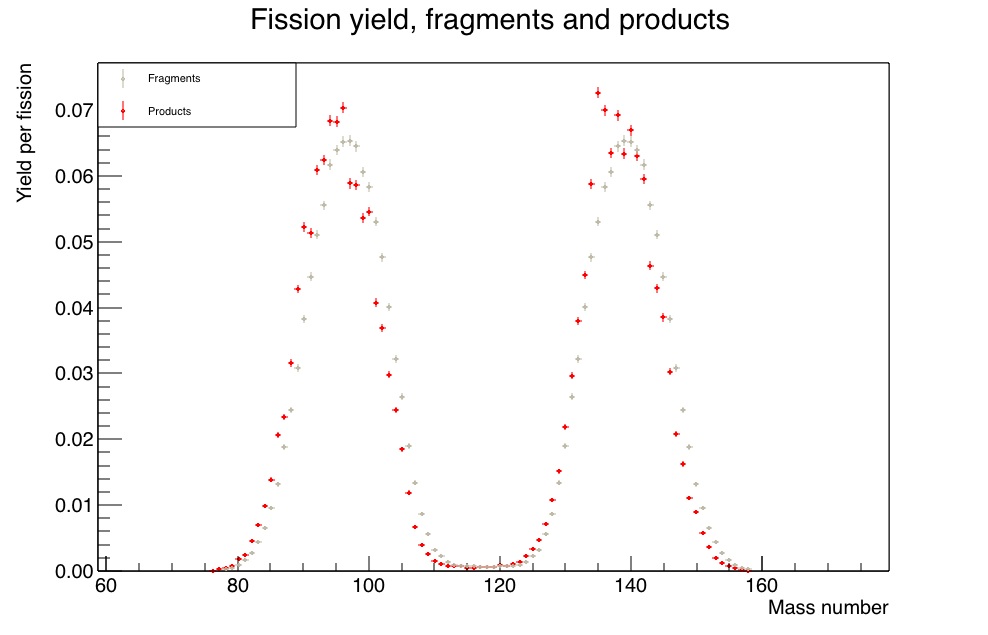
\includegraphics[scale=0.36]{U235_fragment_product_distribution.png}
	\caption{The fragment and product mass distribution from the thermal neutron induced fission of U235}
	\label{fig:U235_fragment_product_distribution}
\end{figure}

\begin{figure} [H]
	\centering
	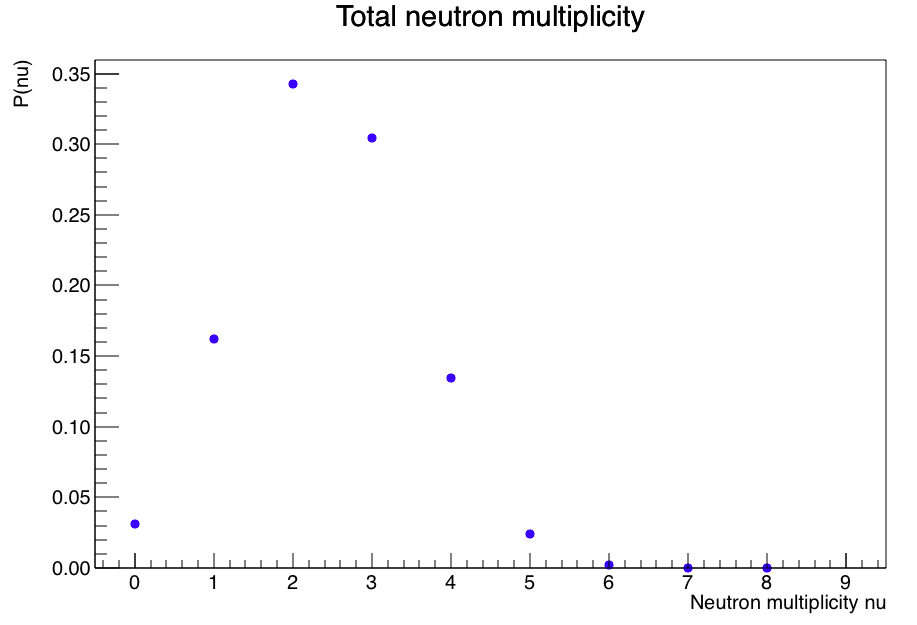
\includegraphics[scale=0.36]{U235_n_mult.png}
	\caption{The multiplicity distribution of neutrons from the thermal neutron-induced fission of U235}
	\label{fig:U235_n_mult}
\end{figure}

\begin{figure} [H]
	\centering
	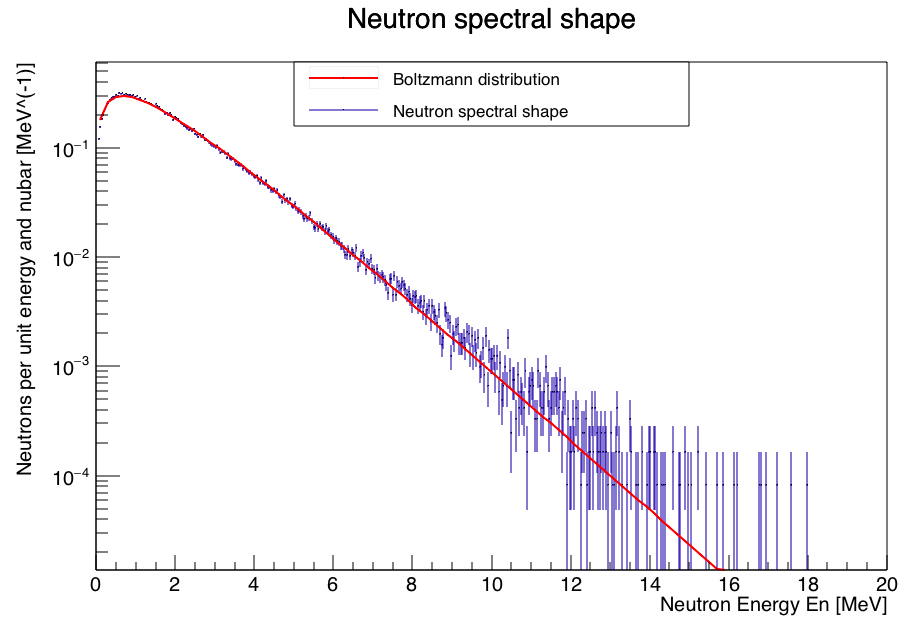
\includegraphics[scale=0.36]{U235_n_spectral_shape.png}
	\caption{The spectral shape of neutrons from the thermal neutron induced fission of U235, compared to a fitted Boltzmann distribution}
	\label{fig:U235_n_spectral_shape}
\end{figure}

\begin{figure} [H]
	\centering
	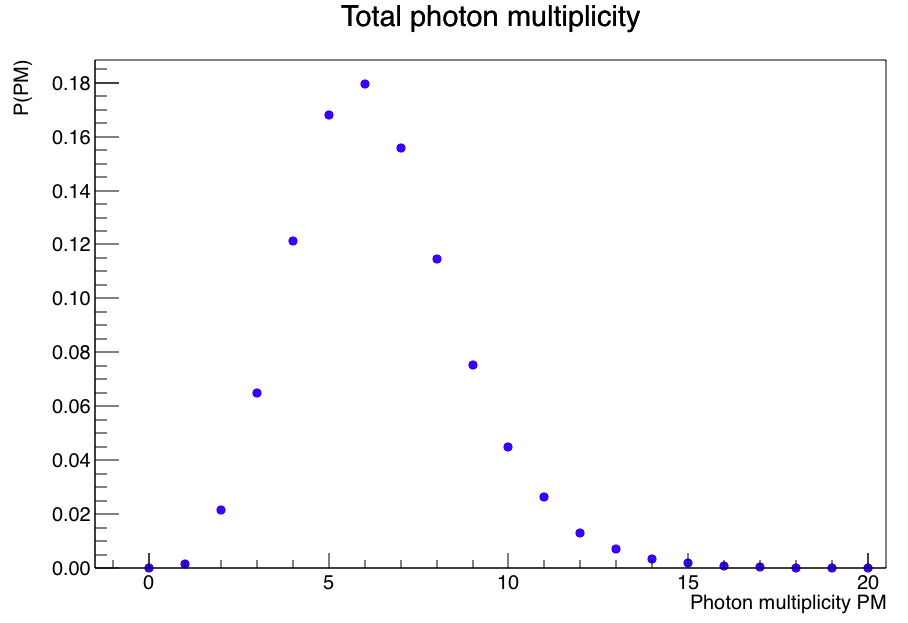
\includegraphics[scale=0.36]{U235_ph_mult.png}
	\caption{The multiplicity distribution of photons from the thermal neutron-induced fission of U235}
	\label{fig:U235_ph_mult}
\end{figure}

\begin{figure} [H]
	\centering
	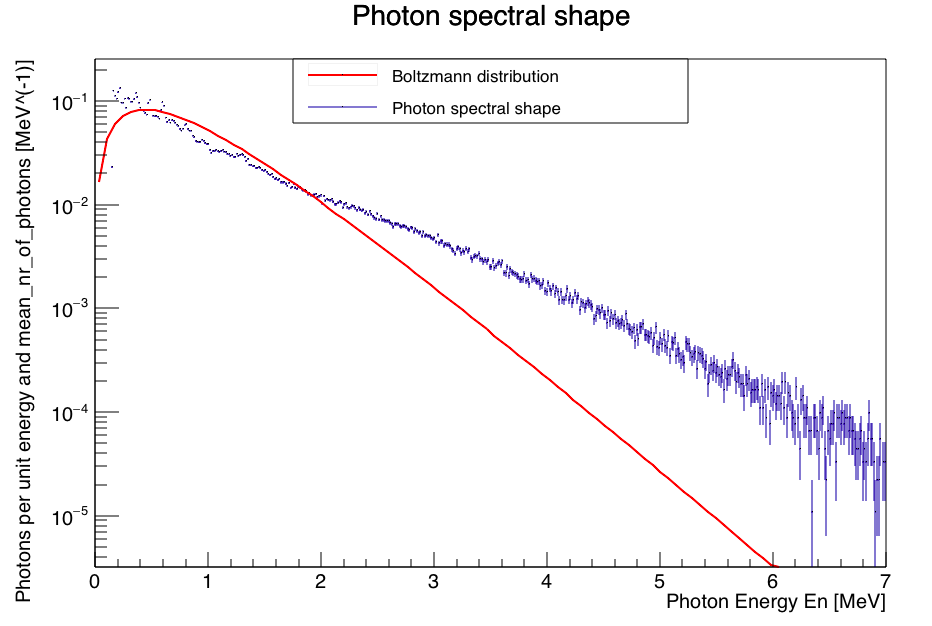
\includegraphics[scale=0.34]{U235_ph_spectral_shape.png}
	\caption{The spectral shape of photons from the thermal neutron induced fission of U235, compared to a fitted Boltzmann distribution}
	\label{fig:U235_ph_spectral_shape}
\end{figure}

\begin{figure} [H]
	\centering
	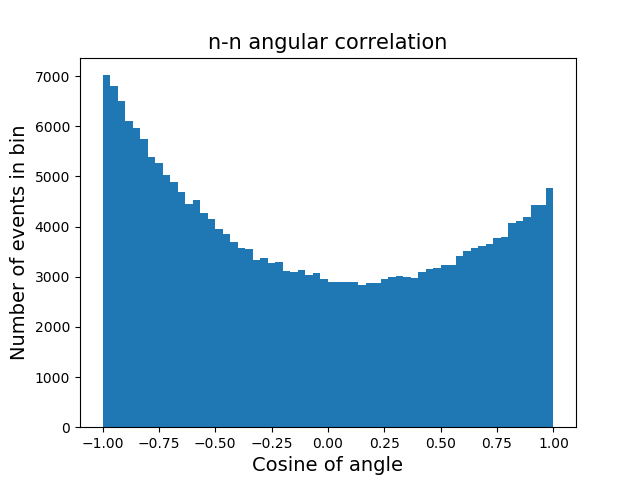
\includegraphics[scale=0.65]{U235_n_n_ang_corr.png}
	\caption{The angulare correlation between pairs of emmited neutrons from the thermal neutron-induced fission of U235}
	\label{fig:U235_n_n_ang_corr}
\end{figure}


\subsection{Neutron induced fission of Pu239}

\begin{table} [H]
	\centering
	\caption{Neutrons, first four factorial moments. From neutron-induced fission of Pu239, with E$_n$ = 0.1 MeV }
	\begin{tabularx}{\textwidth}{XXXXX} \hline
		\label{Pu239_n_moments_0_1}
		Moment & $\nu$ & $\nu_0$ & $\nu_1$ & $\nu_2$ \\ \hline
		1 & 2.89026 & 0 &1.62009 & 1.27017\\
		2 & 6.7476 & 0 & 1.75306 & 0.97784\\
		3 & 12.2142 & 0 & 1.07502 & 0.40332\\
		4 & 16.2727 & 0 & 0.29856 & 0.06936\\ 
	\end{tabularx}
\end{table}

\begin{table} [H]
	\centering
	\caption{Neutrons, first four factorial moments. From neutron-induced fission of Pu239, with E$_n$ = 2.0 MeV }
	\begin{tabularx}{\textwidth}{XXXXX} \hline
		\label{Pu239_n_moments_2}
		Moment & $\nu$ & $\nu_0$ & $\nu_1$ & $\nu_2$ \\ \hline
		1 & 3.13967 & 0.00338 & 1.74664 & 1.39134\\
		2 & 8.12418 & 0 & 2.1249 & 1.24976\\
		3 & 16.7641 & 0 & 1.5852 & 0.65838\\
		4 & 26.4527 & 0 & 0.6012 & 0.18072\\ 
	\end{tabularx}
\end{table}

\begin{table} [H]
	\centering
	\caption{Neutrons, first four factorial moments. From neutron-induced fission of Pu239, with E$_n$ = 8.0 MeV }
	\begin{tabularx}{\textwidth}{XXXXX} \hline
		\label{Pu239_n_moments_8}
		Moment & $\nu$ & $\nu_0$ & $\nu_1$ & $\nu_2$ \\ \hline
		1 & 3.8262 & 0.54674 & 1.97688 & 1.57595\\
		2 & 12.6219 & 0 & 2.9383 & 1.7681\\
		3 & 35.2788 & 0 & 3.09714 & 1.37334\\
		4 & 82.0861 & 0 & 2.2596 & 0.71616\\ 
	\end{tabularx}
\end{table}

\begin{table} [H]
	\centering
	\caption{Neutrons, first four factorial moments. From neutron-induced fission of Pu239, with E$_n$ = 14.0 MeV }
	\begin{tabularx}{\textwidth}{XXXXX} \hline
		\label{Pu239_n_moments_14}
		Moment & $\nu$ & $\nu_0$ & $\nu_1$ & $\nu_2$ \\ \hline
		1 & 4.49802 & 0.93108 & 2.29912 & 1.73344\\
		2 & 18.217 & 0.48466 & 4.32362 & 2.2436\\
		3 & 65.9636 & 0 & 6.57924 & 2.13492\\
		4 & 212.075 & 0 & 8.1756 & 1.45224\\ 
	\end{tabularx}
\end{table}

\begin{table} [H]
	\centering
	\caption{Neutrons, first four factorial moments. From neutron-induced fission of Pu239, with E$_n$ = 20.0 MeV }
	\begin{tabularx}{\textwidth}{XXXXX} \hline
		\label{Pu239_n_moments_20}
		Moment & $\nu$ & $\nu_0$ & $\nu_1$ & $\nu_2$ \\ \hline
		1 & 5.04612 & 1.11361 & 2.57681 & 1.91351\\
		2 & 23.3884 & 0.72198 & 5.61242 & 2.83246\\
		3 & 98.8097 & 0.04158 & 10.1763 & 3.16566\\
		4 & 377.024 & 0 & 15.2033 & Moment4 2.58768\\ 
	\end{tabularx}
\end{table}

\section{Discussion}

\section{Conclusion}

\vspace{3mm}

\end{document} 

